\documentclass[11pt]{article}
\usepackage[margin=0.68in]{geometry}
\usepackage{booktabs}
\usepackage{enumitem}
\usepackage{fancyhdr}
\usepackage{graphicx}
\usepackage[table]{xcolor}
\usepackage[hidelinks]{hyperref}
\usepackage{listings}
\usepackage{microtype}
\usepackage{tabularx}
\usepackage{titlesec}
\graphicspath{{docs/lessons/assets/}{../assets/}}
\definecolor{Ink}{gray}{0}
\definecolor{CodeGray}{gray}{0.96}
\hypersetup{
  pdftitle={ADK Lesson 020: The Direction Chase},
  pdfauthor={Kevin Shanahan},
  pdfsubject={A fast, inert demonstration of bounded motor intent and reversal dead time},
  pdflang={en-US}
}
\pagestyle{fancy}
\fancyhf{}
\lhead{\textsc{ADK Lesson 020}}
\rhead{The Direction Chase}
\cfoot{\thepage}
\setlength{\headheight}{14pt}
\setlength{\parindent}{0pt}
\setlength{\parskip}{5pt}
\setlist{nosep,leftmargin=1.45em}
\titleformat{\section}{\Large\bfseries\color{Ink}}{\thesection}{0.5em}{}
\lstdefinestyle{adkcpp}{
  language=C++,backgroundcolor=\color{CodeGray},basicstyle=\ttfamily\small,
  keywordstyle=\color{Ink}\bfseries,columns=fullflexible,keepspaces=true,
  showstringspaces=false,frame=single,rulecolor=\color{Ink},breaklines=true
}
\newcommand{\lessonbox}[1]{\begin{center}\fbox{\parbox{0.92\linewidth}{#1}}\end{center}}

\begin{document}
\begin{center}
  {\Huge\bfseries The Direction Chase}\\[4pt]
  {\Large Three lamps race, reverse, and shut themselves down}\\[7pt]
  \textit{Motor logic you can see, with no motor or driver connected.}
\end{center}

\begin{tabularx}{\linewidth}{@{}>{\bfseries}l X >{\bfseries}l X@{}}
Lesson & 020 --- component & Build time & about 20 minutes\\
Board & Arduino Mega 2560 & Power & USB only\\
Visible result & two direction rounds & Finish & automatic at 10 seconds\\
\end{tabularx}

\section{What you are making}

Three LEDs stand in for the inputs of a future motor driver. Forward and
reverse are direction lamps. Enable is the ``go'' lamp: its brightness changes
with PWM duty. On every reversal all three go dark for 250 ms before the other
direction may light.

\lessonbox{\textbf{The whole lesson is inert.} Use only the three LEDs and
resistors shown here. Do not connect an H-bridge, motor, motor supply, relay, or
wheel. The Elegoo family listing does not establish an exact driver or motor
electrical identity, so powered motion is outside this lesson.}

\section{Parts}

\begin{tabularx}{\linewidth}{@{}l X@{}}
\toprule
Part & Use\\
\midrule
Arduino Mega 2560 & runs the fixed ten-second show\\
Three ordinary LEDs & forward, reverse, and enable lamps\\
Three 1 k\(\Omega\) resistors & one series resistor for each LED\\
Breadboard and jumpers & the three independent signal paths\\
\bottomrule
\end{tabularx}

At a conservative 5 V rail and 2 V LED drop, each continuously lit path is
about \((5-2)/1000=3\) mA. Unplug USB before changing a wire. If an LED is hot,
the USB connection is unstable, or the picture and your board disagree,
unplug and inspect the circuit.

\newpage
\section{Find the exact pins}

On the Mega's long paired digital header, find D22 and D23 next to each other.
D6 is on the PWM-numbered digital header near the board end. Use any labeled
GND pin. The drawing separates these locations so the labels remain readable.

\begin{center}
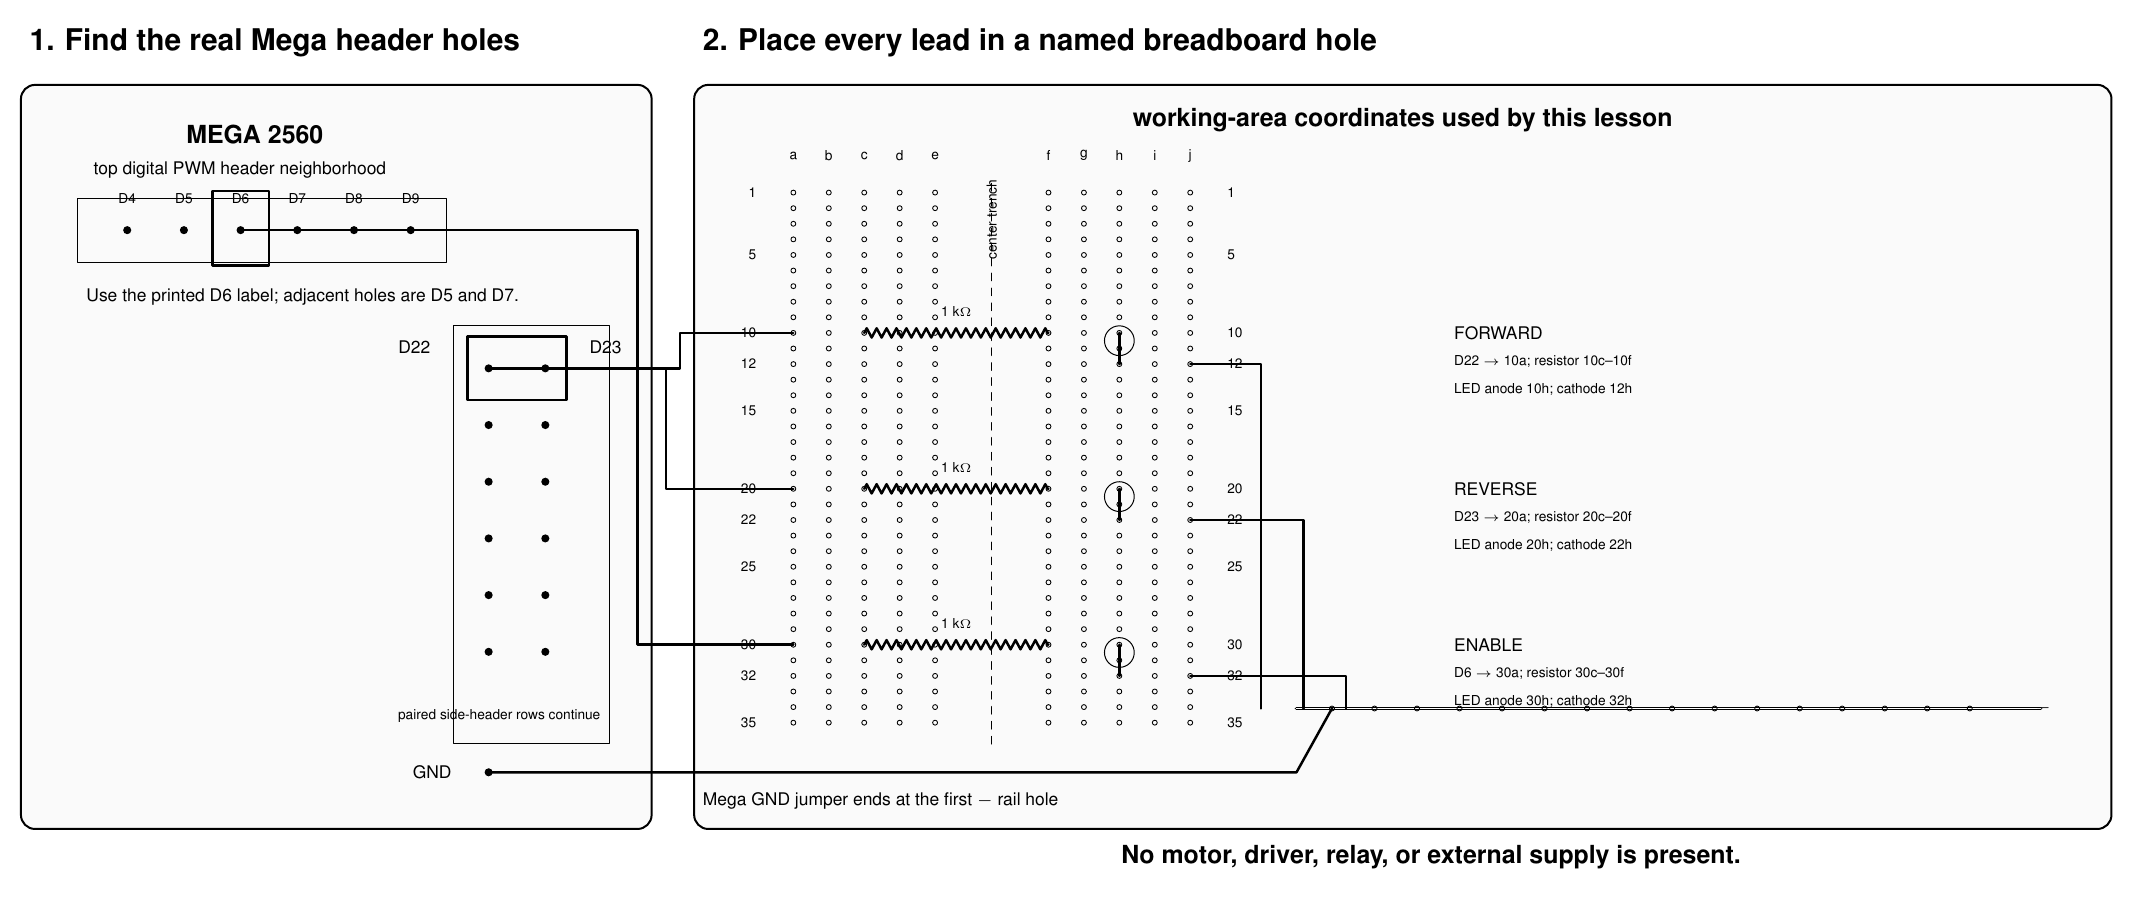
\includegraphics[width=0.98\linewidth]{020-motor-intent-layout.png}

\small\textit{A pencil-style layout of the Mega paired header and breadboard.
D22, D23, and D6 each run through their own 1 k\(\Omega\) resistor to an LED
long leg. All three short legs return through the breadboard negative rail to
Mega GND. No motor or driver appears in the circuit.}
\end{center}

\begin{tabularx}{\linewidth}{@{}l l X@{}}
\toprule
Lamp & Mega pin & Complete electrical path\\
\midrule
Forward / TP-F & D22 & D22 \(\rightarrow\) 1 k\(\Omega\)
  \(\rightarrow\) LED long leg; short leg \(\rightarrow\) negative rail\\
Reverse / TP-R & D23 & D23 \(\rightarrow\) 1 k\(\Omega\)
  \(\rightarrow\) LED long leg; short leg \(\rightarrow\) negative rail\\
Enable / TP-E & D6 & D6 \(\rightarrow\) 1 k\(\Omega\)
  \(\rightarrow\) LED long leg; short leg \(\rightarrow\) negative rail\\
Return & GND & Mega GND \(\rightarrow\) negative rail\\
\bottomrule
\end{tabularx}

\section{Build in three payoffs}

\textbf{First payoff --- direction.} Build only D22 and its LED path, then add
D23 and its path. The two LEDs must have separate resistors. A shared resistor
would couple the signals and spoil the chase.

\textbf{Second payoff --- speed.} Add D6 and the enable LED. This lamp starts
dim, becomes bright, and later runs bright in both directions. That visible
change comes from two same-direction duty commands, not from a delay.

\textbf{Third payoff --- reversal.} Upload the canonical sketch. Watch closely
when forward hands the chase to reverse: every lamp goes dark before reverse
and enable return. The reverse round cannot appear correctly unless both
direction paths and enable are independent.

\newpage
\section{Read the ten-second show}

\begin{tabularx}{\linewidth}{@{}r l l X@{}}
\toprule
Time & Direction lamps & Enable lamp & What the controller is doing\\
\midrule
0.00--0.75 s & both dark & dark & stopped and ready\\
0.75--1.75 s & forward & dim & forward at duty 72\\
1.75--2.75 s & forward & bright & same direction, duty 180\\
2.75 s & both dark & dark & 250 ms reversal dead time\\
about 3.00--4.50 s & reverse & bright & reverse at duty 160\\
4.50--5.50 s & both dark & dark & stopped between rounds\\
5.50--6.50 s & forward & bright & second round\\
6.50 s & both dark & dark & another 250 ms dead time\\
about 6.75--8.00 s & reverse & bright & second reversal completed\\
8.00--10.00 s & both dark & dark & stopped\\
10.00 s onward & all dark & dark & automatic safe shutdown\\
\bottomrule
\end{tabularx}

The blackout is the important trick. The requested direction may already be
reverse while the \emph{applied} command remains stopped. The opposite output
is allowed only after the explicit deadline.

\begin{lstlisting}[style=adkcpp]
void loop ()
{
    const adk::TimePoint now (millis ());

    observeOperatorRequest (now);
    decideMotorIntent      (now);
    actuateMotorEvidence   ();
}
\end{lstlisting}

The loop always observes, decides, then actuates the applied snapshot. There is
no blocking delay. Stop cancels pending motion, no state permits both direction
signals high, and shutdown first requests stopped intent before releasing the
pins.

\section{Make the idea your own}

\begin{enumerate}
  \item Swap the physical forward and reverse LEDs. Predict how the show will
    look while the code's meaning stays unchanged.
  \item Change the first duty from 72 to 36. The enable lamp should begin even
    dimmer, while direction remains forward.
  \item Change the dead time from 250 ms to 500 ms. The deliberate blackout
    becomes much easier to count.
  \item Add a third round that requests stop during the blackout. A correct
    controller stays dark instead of restarting at the old deadline.
\end{enumerate}

\section{If the chase looks wrong}

\begin{tabularx}{\linewidth}{@{}l X@{}}
\toprule
What you see & Inspect while USB is unplugged\\
\midrule
One direction never lights & its LED polarity and its pin--resistor--LED path\\
Both directions light together & accidental shared rows or a D22/D23 short\\
Direction works but enable is dark & D6 path, LED polarity, and resistor row\\
No brightness change & confirm the enable jumper really starts at PWM pin D6\\
No dark reversal gap & confirm you uploaded the Lesson 020 sketch\\
Lights remain after 10 seconds & reset once; if repeated, disconnect USB\\
\bottomrule
\end{tabularx}

\section{What the repository checks behind the scenes}

Automated tests replay stopped, same-direction speed changes, both reversals,
stop during dead time, exact deadline edges, time wraparound, invalid commands,
rollback, repeated shutdown, and resource reuse. The Mega build also checks
the sketch's flash and RAM budget. Those checks protect the lesson; they are
not extra chores for the learner.

\section{Where this leads}

A real motor needs an exactly identified motor, driver, primary datasheets,
measured stall current, separate current-limited load supply, complete flyback
path, physical power disconnect, and guarded unloaded fixture. None of those
facts follows from a retail kit-family name. Until that separate E2 work is
qualified, these three lamps are the complete supported circuit.

\vfill
\small
Status: host verified; physical observation remains unclaimed. Current
reference material and the canonical sketch are published with the HTML
lesson.
\end{document}
